\let\negmedspace\undefined
\let\negthickspace\undefined
\documentclass[journal]{IEEEtran}
\usepackage[a5paper, margin =  10mm, onecolumn]{geometry}
%\usepackage{lmodern} % Ensure lmodern is loaded for pdflatex
\usepackage{tfrupee} % Include tfrupee package

\setlength{\headheight}{1cm} % Set the height of the header box
\setlength{\headsep}{0mm}     % Set the distance between the header box and the top of the text

\usepackage{gvv-book}
\usepackage{gvv}
\usepackage{cite}
\usepackage{amsmath,amssymb,amsfonts,amsthm}
\usepackage{algorithmic}
\usepackage{graphicx}
\usepackage{textcomp}
\usepackage{xcolor}
\usepackage{txfonts}
\usepackage{listings}
\usepackage{enumitem}
\usepackage{mathtools}
\usepackage{gensymb}
\usepackage{comment}
\usepackage[breaklinks =  true]{hyperref}
\usepackage{tkz-euclide} 
\usepackage{listings}
% \usepackage{gvv}                                        
\def\inputGnumericTable{}                                 
\usepackage[latin1]{inputenc}                                
\usepackage{color}                                            
\usepackage{array}                                            
\usepackage{longtable}                                       
\usepackage{calc}                                             
\usepackage{multirow}                                         
\usepackage{hhline}                                           
\usepackage{ifthen}                                           
\usepackage{lscape}
\begin{document}

\bibliographystyle{IEEEtran}
\vspace{1cm}

\title{4.7.26}
\author{EE25BTECH11034 - Kishora Karthik}
% \maketitle
% \newpage
% \bigskip
{\let\newpage\relax\maketitle}

\renewcommand{\thefigure}{\theenumi}
\renewcommand{\thetable}{\theenumi}
%\setlength{\intextsep}{10pt} % Space between text and floats
\textbf{Question:}\\
Find the equation of a straight line on which length of perpendicular from the origin is four units and the line makes an angle of $120\degree$ with the positive direction of X-axis.
\\

\textbf{Solution:}\\
Let $p$ be the length of perpendicular from the origin and $\theta$ be the angle made by the line with the positive X-axis.\\
Given, $p=4$ and $\theta=120\degree$.
Let the angle made by the perpendicular with the positive X-axis be $\alpha$.
\begin{align}
    \alpha=90\degree-(180\degree-\theta)
\end{align}
\begin{align}
    \alpha=90\degree-(180\degree-120\degree)
\end{align}
\begin{align}
    \alpha=30\degree
\end{align}
$p\myvec{ \cos\alpha \\ \sin\alpha }$
is a point on the line as well as the normal vector. Hence the equation of the line is,
\begin{align}
p\myvec{ \cos\alpha \\ \sin\alpha}^\top\brak{\vec{x} - p  \myvec{ \cos\alpha \\ \sin\alpha}}   = 0
\end{align}
\begin{align}
\implies p\myvec{ \cos\alpha & \sin\alpha}\brak{\vec{x} - p  \myvec{ \cos\alpha \\ \sin\alpha}}   = 0
\end{align}
\begin{align}
\implies  p\myvec{ \cos\alpha & \sin\alpha}\vec{x} = p^2(\cos^2\alpha+\sin^2\alpha) 
\end{align}
\begin{align}
\implies  \myvec{ \cos\alpha & \sin\alpha}\vec{x} = p 
\end{align}
So the equation of the straight line is,
\begin{align}
\myvec{ \cos30\degree & \sin30\degree}\vec{x} = 4 
\end{align}
\begin{align}
\myvec{ \frac{\sqrt{3}}{2} & \frac{1}{2}}\vec{x} = 4 
\end{align}
$\therefore$ The equation of the required line is $\myvec{ \frac{\sqrt{3}}{2} & \frac{1}{2}}\vec{x} = 4$ or ${\sqrt{3}}x + y=8$.
\centering   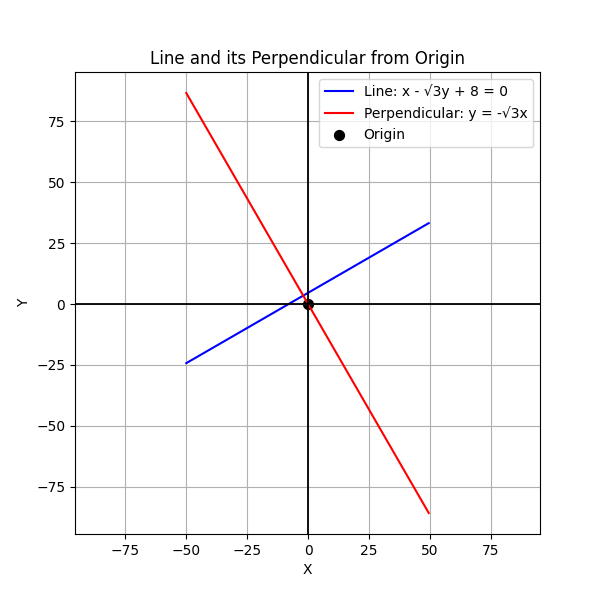
\includegraphics[width=\columnwidth, height=1\textheight, keepaspectratio]{figs/fig1.png}

\end{document}
